\section{Graphing a Linear Equation}

In this section, you will learn to:

\begin{enumerate}
    \item Graph a line when you know its equation.
    \item Graph a line when you are given its equation in parametric form.
    \item Graph and find equations of vertical and horizontal lines.
\end{enumerate}

\subsection{Graphing a Line from its Equation}

Equations whose graphs are straight lines are called linear equations. The following are some examples of linear equations:

\begin{align*}
2x - 3y &= 6, \\
3x &= 4y - 7, \\
y &= 2x - 5, \\
2y &= 3, \\
x - 2 &= 0.
\end{align*}

A line is completely determined by two points. Therefore, to graph a linear equation, we need to find the coordinates of two points. This can be accomplished by choosing an arbitrary value for x or y and then solving for the other variable.

\begin{example}
Graph the line \(y = 3x + 2\).
\end{example}

\begin{solution} We need to find the coordinates of at least two points. We arbitrarily choose \(x = -1\), \(x = 0\), and \(x = 1\).

If \(x = -1\), then \(y = 3(-1) + 2\) or \(y = -1\). Therefore, \((-1, -1)\) is a point on this line.

If \(x = 0\), then \(y = 3(0) + 2\) or \(y = 2\). Hence the point \((0, 2)\).

If \(x = 1\), then \(y = 5\), and we get the point \((1, 5)\). Below, the results are summarized, and the line is graphed.

\begin{center}
\begin{tabular}{c|c}
    \(x\) & \(y\) \\
    \hline
    -1 & -1 \\
    0  & 2  \\
    1  & 5
\end{tabular}
\end{center}


\begin{center}
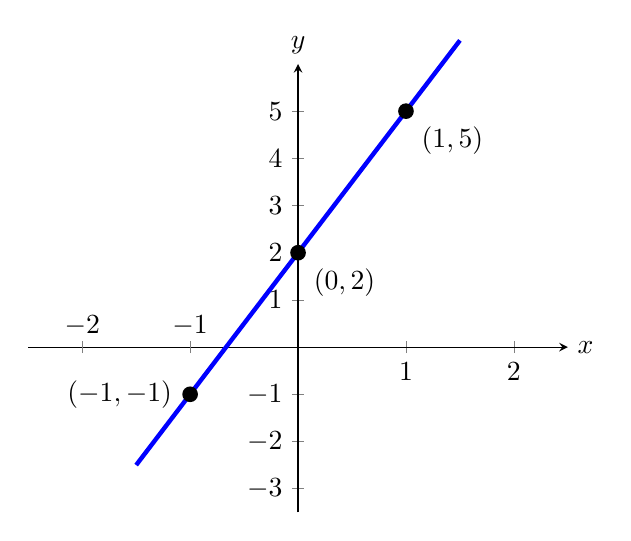
\begin{tikzpicture}
\begin{axis}[
    axis lines=middle,
    xlabel={$x$},
    ylabel={$y$},
    xlabel style={anchor=west},
    ylabel style={anchor=south},
    xmin=-2.5, xmax=2.5,
    ymin=-3.5, ymax=6,
    xtick={0,1,...,2},
		% to flip a couple ticks to the top of the x axis use the next 2 lines
		extra x ticks={-2,-1}, 
    extra x tick style={tick label style={yshift=1mm,anchor=south}},
    ytick={-3,-2,...,5},
    clip=false
]

% Update the line equation and domain to cover the new points
\addplot[blue, ultra thick, domain=-1.5:1.5] {3*x + 2};

% Update the points and their labels
\node[label={left:{$(-1,-1)$}}, ,circle,fill,inner sep=2pt] at (axis cs:-1,-1) {};
\node[label={below right:{$(0,2)$}},circle,fill,inner sep=2pt] at (axis cs:0,2) {};
\node[label={below right:{$(1,5)$}},circle,fill,inner sep=2pt] at (axis cs:1,5) {};

\end{axis}
\end{tikzpicture}
\end{center}


\end{solution}

\begin{example}
Graph the line: $2x + y = 4$
\end{example}

\begin{solution} Again, we need to find coordinates of at least two points. We arbitrarily choose $x = -1$, $x = 0$, and $y = 2$.

If $x = -1$, then $2(-1) + y = 4$ which results in $y = 6$. Therefore, $(-1, 6)$ is a point on this line.

If $x = 0$, then $2(0) + y = 4$, which results in $y = 4$. Hence the point $(0, 4)$.

If $y = 2$, then $2x + 2 = 4$, which yields $x = 1$, and gives the point $(1, 2)$. The table below shows the points, and the line is graphed.

\begin{center}
\begin{tabular}{c|c}
    $x$ & $y$ \\
    \hline
    $-1$ & $6$ \\
    $0$  & $4$ \\
    $1$  & $2$
\end{tabular}
\end{center}

\begin{center}
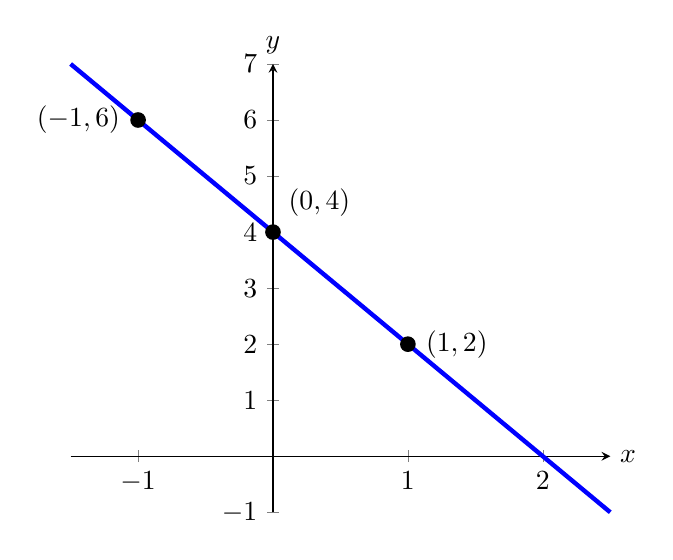
\begin{tikzpicture}
\begin{axis}[
    axis lines=middle,
    xlabel={$x$},
    ylabel={$y$},
    xlabel style={anchor=west},
    ylabel style={anchor=south},
    xmin=-1.5, xmax=2.5,
    ymin=-1, ymax=7,
    xtick={-1,0,...,2},
    ytick={-1,0,...,7},
    clip=false
]

% Draw the line through (-1,6), (0,4), and (1,2)
\addplot[blue, ultra thick, domain=-1.5:2.5] {-2*x + 4};

% Mark the points
\node[label={left:{$(-1,6)$}},circle,fill,inner sep=2pt] at (axis cs:-1,6) {};
\node[label={above right:{$(0,4)$}},circle,fill,inner sep=2pt] at (axis cs:0,4) {};
\node[label={right:{$(1,2)$}},circle,fill,inner sep=2pt] at (axis cs:1,2) {};

\end{axis}
\end{tikzpicture}
\end{center}


\end{solution}

\subsection{Intercepts:} The points at which a line crosses the coordinate axes are called the intercepts. When graphing a line by plotting two points, using the intercepts is often preferred because they are easy to find.
\begin{itemize}
    \item To find the value of the x-intercept, we let $y = 0$.
    \item To find the value of the y-intercept, we let $x = 0$.
\end{itemize}

\begin{example}
Find the intercepts of the line: $2x - 3y = 6$, and graph.
\end{example}

\begin{solution} To find the x-intercept, let $y = 0$ in the equation, and solve for $x$.
\begin{align*}
2x - 3(0) &= 6 \\
2x &= 6 \\
x &= 3
\end{align*}
Therefore, the x-intercept is the point $(3, 0)$.

To find the y-intercept, let $x = 0$ in the equation, and solve for $y$.
\begin{align*}
2(0) - 3y &= 6 \\
0 - 3y &= 6 \\
-3y &= 6 \\
y &= -2
\end{align*}
Therefore, the y-intercept is the point $(0, -2)$.

To graph the line, plot the points for the x-intercept $(3, 0)$ and the y-intercept $(0, -2)$, and use them to draw the line.

\begin{center}
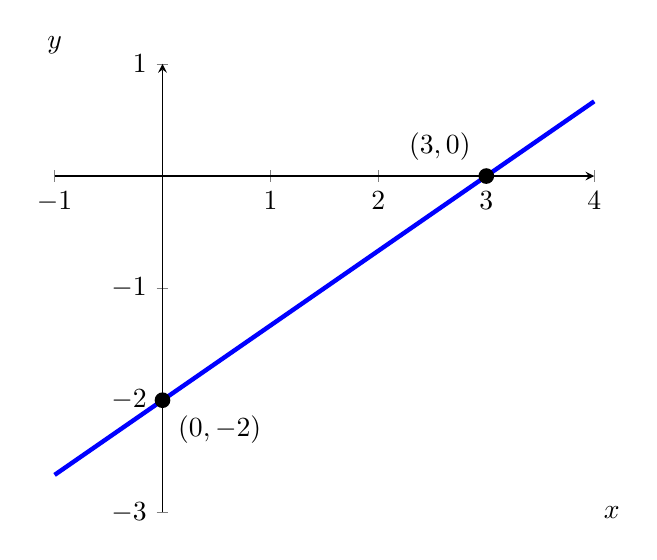
\begin{tikzpicture}
\begin{axis}[
    axis lines=middle,
    xlabel={$x$},
    ylabel={$y$},
    xlabel style={at={(rel axis cs:1,0)},anchor=west},
    ylabel style={at={(rel axis cs:0,1)},anchor=south},
    xmin=-1, xmax=4,
    ymin=-3, ymax=1,
    xtick={-1,0,...,4},
    ytick={-3,-2,...,1},
    clip=false
]

% Draw the line through (0,-2) and (3,0)
\addplot[blue, ultra thick, domain=-1:4] {2/3*x - 2};

% Mark the points
\node[label={below right:{$(0,-2)$}},circle,fill,inner sep=2pt] at (axis cs:0,-2) {};
\node[label={above left:{$(3,0)$}},circle,fill,inner sep=2pt] at (axis cs:3,0) {};

\end{axis}
\end{tikzpicture}
\end{center}


\end{solution}
\subsection{Graphing a Line from Its Equation in Parametric Form}

In higher math, equations of lines are sometimes written in parametric form. For example, $x = 3 + 2t, y = 1 + t$. The letter $t$ is called the parameter or the dummy variable.

Parametric lines can be graphed by finding values for $x$ and $y$ by substituting numerical values for $t$. Plot the points using their $(x, y)$ coordinates and use the points to draw the line.

\begin{example}
Graph the line given by the parametric equations: $x = 3 + 2t$, $y = 1 + t$
\end{example}

\begin{solution} Let $t = 0, 1$ and $2$; for each value of $t$, find the corresponding values for $x$ and $y$. The results are given in the table below.

\begin{center}
\begin{tabular}{c|c|c}
    $t$ & $x$ & $y$ \\
    \hline
    $0$ & $3$ & $1$ \\
    $1$ & $5$ & $2$ \\
    $2$ & $7$ & $3$ \\
\end{tabular}
\end{center}

\begin{center}
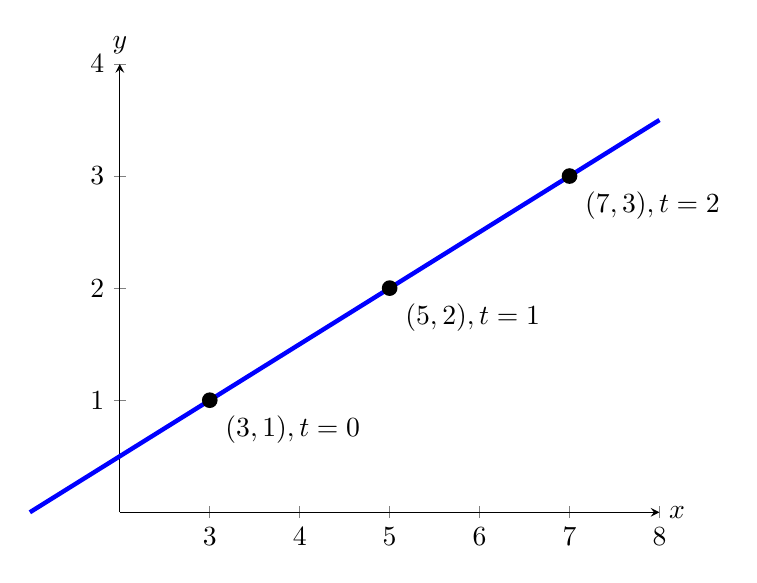
\begin{tikzpicture}
\begin{axis}[
    axis lines=middle,
    xlabel={$x$},
    ylabel={$y$},
    xlabel style={at={(rel axis cs:1,0)},anchor=west},
    ylabel style={at={(rel axis cs:0,1)},anchor=south},
    xmin=2, xmax=8,
    ymin=0, ymax=4,
    xtick={2,3,...,8},
    ytick={0,1,...,4},
    clip=false
]

% Define points based on t values
\coordinate (A) at (3,1);
\coordinate (B) at (5,2);
\coordinate (C) at (7,3);

% Draw the line
\addplot[blue, ultra thick, domain=-2:5] ({x+3},{x/2+1});

% Mark the points and label with coordinates and t values
\node[label={below right:{$(3,1), t=0$}},circle,fill,inner sep=2pt] at (A) {};
\node[label={below right:{$(5,2), t=1$}},circle,fill,inner sep=2pt] at (B) {};
\node[label={below right:{$(7,3), t=2$}},circle,fill,inner sep=2pt] at (C) {};

\end{axis}
\end{tikzpicture}
\end{center}

\end{solution}
\subsection{Horizontal and Vertical Lines}

When an equation of a line has only one variable, the resulting graph is a horizontal or a vertical line.

The graph of the line \(x = a\), where \(a\) is a constant, is a vertical line that passes through the point \((a, 0)\). Every point on this line has the \(x\)-coordinate equal to \(a\), regardless of the \(y\)-coordinate.

The graph of the line \(y = b\), where \(b\) is a constant, is a horizontal line that passes through the point \((0, b)\). Every point on this line has the \(y\)-coordinate equal to \(b\), regardless of the \(x\)-coordinate.

\begin{example}
Graph the lines: \(x = -2\), and \(y = 3\).
\end{example}

\begin{solution} The graph of the line \(x = -2\) is a vertical line that has the \(x\)-coordinate \(-2\) no matter what the \(y\)-coordinate is. The graph is a vertical line passing through point \((-2, 0)\).

\begin{center}
\begin{tikzpicture}
\begin{axis}[
    axis lines=middle,
    xlabel={$x$},
    ylabel={$y$},
    xlabel style={at={(rel axis cs:1,0)},anchor=west},
    ylabel style={at={(rel axis cs:0,1)},anchor=south},
    xmin=-3, xmax=5,
    ymin=-2, ymax=4,
    xtick={-3,-2,...,5},
    ytick={-2,-1,...,4},
    clip=false
]

% Draw the line
\addplot[blue, ultra thick, -] coordinates {(-2,4) (-2,-2)};

% Mark the points
\node[label={above left:{$(-2,0)$}},circle,fill,inner sep=2pt] at (-2,0) {};

\end{axis}
\end{tikzpicture}
\end{center}

The graph of the line \(y = 3\) is a horizontal line that has the \(y\)-coordinate \(3\) regardless of what the \(x\)-coordinate is. Therefore, the graph is a horizontal line that passes through point \((0, 3)\).

\begin{center}
\begin{tikzpicture}
\begin{axis}[
    axis lines=middle,
    xlabel={$x$},
    ylabel={$y$},
    xlabel style={at={(rel axis cs:1,0)},anchor=west},
    ylabel style={at={(rel axis cs:0,1)},anchor=south},
    xmin=-3, xmax=5,
    ymin=-2, ymax=4,
    xtick={-3,-2,...,5},
    ytick={-2,-1,...,4},
    clip=false
]

% Draw the line
\addplot[blue, ultra thick, -] coordinates {(-3,3) (5,3)};

% Mark the points
\node[label={above right:{$(0, 3)$}},circle,fill,inner sep=2pt] at (0, 3) {};

\end{axis}
\end{tikzpicture}
\end{center}

\end{solution}

